\phantomsection\numberedsection{RF1.9.1 Exportar informe de cuenta}

\subsection*{Descripción}
El sistema exporta el informe con la información de la cuenta, incluyendo el
nombre de la cuenta, fecha y hora de creación, número de productos, categorías 
de producto, atributos de usuario y relaciones creadas en formato JSON y se guarda 
de manera local en una ruta escogida por el usuario.

\vspace{0.15cm}

\textbf{Pre-condición}\par
El usuario ha iniciado sesión en Mini PIM, es la cuenta Owner y ya ha creado previamente el informe de cuenta.\par
\vspace{0.15cm}

\textbf{Post-condición}
\begin{itemize}
    \item Caso de éxito: El sistema exporta el informe en formato JSON.
    \item Caso de mínimo: El sistema notifica al usuario el resultado al intentar exportar el informe: exitosa o fallida.
\end{itemize}

\textbf{Prioridad:}
Baja
\vspace{0.15cm}

\textbf{Autores: }
Francisco Javier Jordá Garay y Janine Olegario.\par
\vspace{0.15cm}

\textbf{Control de cambios: } Versión 1: Definición del caso de uso

\numberedsubsection{Escenario principal}
\begin{enumerate}
    \item El usuario ha iniciado sesión con su cuenta Owner.
    \item El usuario accede a la sección de \enquote{Cuenta}.
    \item El usuario selecciona la opción \enquote{Exportar informe}.
    \item El sistema muestra el menú de previsualización del JSON donde el usuario escoge la ruta donde quiere guardar el informe.
    \item El sistema exporta el informe con los datos de la cuenta del usuario en formato JSON.
    \item El sistema guarda el archivo de manera local en el equipo del usuario en la ruta especificada.
\end{enumerate}

\numberedsubsection{Escenarios alternativos}
\begin{description}
    \item[3.a] Se produce un error en el sistema que no permite la exportación del informe.
    \begin{enumerate}
        \item[3.a.1] El sistema muestra un mensaje indicando que se ha producido un error.
        \item[3.a.2] El sistema vuelve al apartado \enquote{Cuenta}.
    \end{enumerate}

    \newpage % Para que el escenario 4.a se vea completo en una página

    \item[4.a] El usuario elige una ruta local inválida.
    \begin{enumerate}
        \item[4.a.1] El sistema muestra un mensaje de error indicando que la ruta es inválida\footnote{Una ruta inválida es una que no exista en el ordenador del usuario o una que no tenga permisos de escritura.}.
        \item[4.a.2] El sistema permite al usuario cambiar la ruta en el menú de previsualización del JSON.
    \end{enumerate}

\end{description}

\numberedsubsection{Casos de Prueba}
\underline{Escenario: Principal}\par
\vspace{0.15cm}
\textbf{Dado} que el usuario ha iniciado sesión con su cuenta Owner,\par 
\textbf{Y} accede a la sección \enquote{Cuenta},\par 
\textbf{Cuando} selecciona la opción \enquote{Exportar informe},\par
\textbf{Y} el sistema muestra el menú de previsualización del JSON,\par
\textbf{Y} el usuario escoge la ruta donde quiere guardar el informe,\par
\textbf{Entonces} el sistema exporta el archivo en formato JSON con los datos de la cuenta del usuario,\par
\textbf{Y} lo guarda localmente en el equipo en la ruta especificada.\par
\vspace{0.20cm}

\underline{Escenario: 2.a (Error en la exportación)}\par
\vspace{0.15cm}
\textbf{Dado} que el usuario ha iniciado sesión con su cuenta Owner,\par 
\textbf{Y} accede a la sección \enquote{Cuenta},\par 
\textbf{Cuando} selecciona la opción \enquote{Exportar informe}, \par
\textbf{Y} se produce un error en el sistema,\par
\textbf{Entonces} el sistema muestra un mensaje de error indicando que no se pudo completar la exportación,\par
\textbf{Y} redirige al usuario al apartado \textit{Cuenta}.\par
\vspace{0.20cm}

\underline{Escenario: 3.a (Ruta inválida)}\par
\vspace{0.15cm}
\textbf{Dado} que el usuario ha iniciado sesión con su cuenta de Owner,\par 
\textbf{Y} accede a la sección \enquote{Cuenta},\par 
\textbf{Cuando} selecciona la opción \enquote{Exportar informe},\par
\textbf{Y} el sistema muestra el menú de previsualización del JSON,\par
\textbf{Y} el usuario introduce una ruta de archivo local inválida,\par
\textbf{Entonces} el sistema muestra un mensaje de error indicando que la ruta no es válida,\par
\textbf{Y} redirige al usuario al al menú de previsualización del JSON,\par
\textbf{Y} le permite cambiar la ruta.\par
\vspace{0.20cm}

\newpage % Mostramos los bocetos en una nueva página

\numberedsubsection{Bocetos}
\begin{figure}[H]
    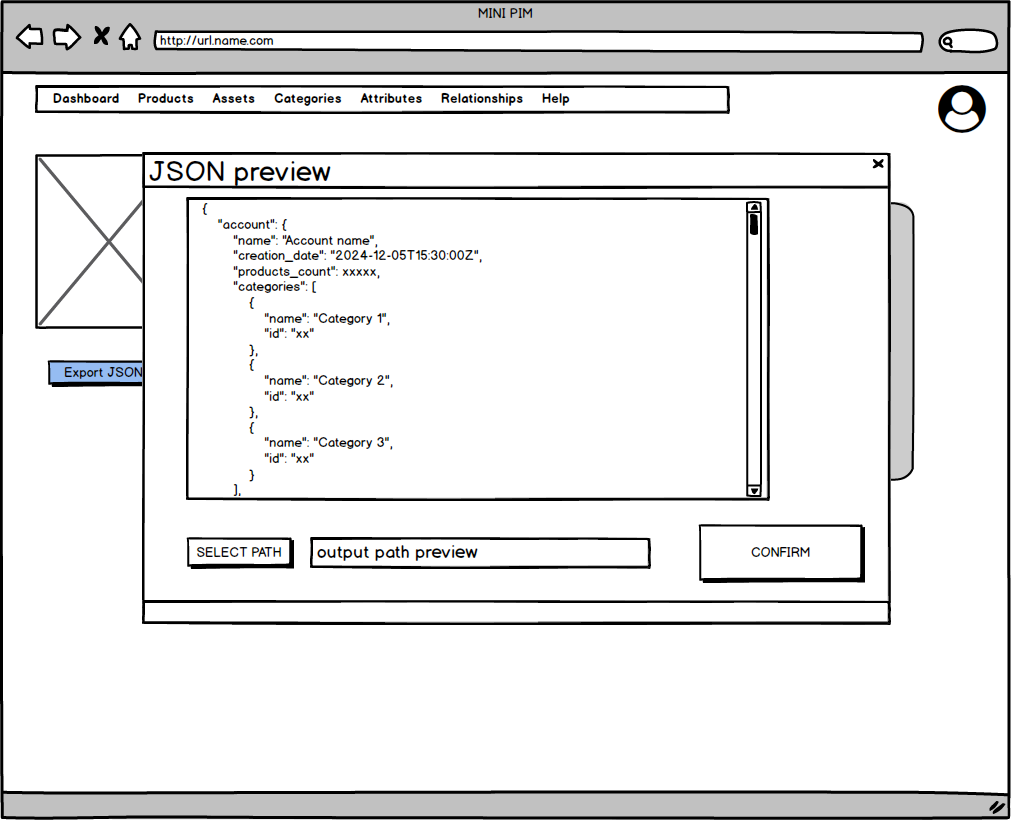
\includegraphics[width=1\linewidth]{mockups/RF1.9.1ExportarInformeCuenta.png}
    \caption{Menú de previsualización del JSON tras clicar \enquote{Export JSON}}
   \end{figure}
\vspace{1.0cm}

\newpage %Inicia en una nueva página otro caso de uso